\documentclass[a4paper,10pt,oneside,onecolumn]{book}

\setlength{\textwidth}{160mm}
\setlength{\textheight}{260mm}
\setlength{\oddsidemargin}{-0cm}
\setlength{\evensidemargin}{28mm}
%\setlength{\topmargin}{-2cm}

\usepackage[
top    = 2.75cm,
bottom = 2.50cm,
left   = 3.00cm,
right  = 2.50cm]{geometry}

\usepackage[spanish]{babel}
\usepackage[utf8]{inputenc}
\usepackage[T1]{fontenc}
\usepackage{textcomp}
\usepackage{lmodern}

\usepackage{amsmath,amssymb}
\usepackage{latexsym}
\usepackage{makebox}
\usepackage{fancyhdr}

\usepackage{float}
\usepackage{graphicx}
\usepackage{epsfig} 

\title{Anàlisis Matemàtico I}
\author{
Facundo Beltramo\\
contacto: fexbef[arroba]gmail.com
}
\date{Fecha: xx de xx del 20xx}


\pagestyle{fancy} 
%\lhead{Consejos para comprar una Computadora}
\rhead{lalala}
\renewcommand{\headrulewidth}{0.4pt} % grosor de la línea de la cabecera

\setcounter{secnumdepth}{3} % para que ponga 1.1.1.1 en subsubsecciones...
\setcounter{tocdepth}{4} % para que añada las subsubsecciones y párrafos en el indice...

\begin{document}
\maketitle
\tableofcontents % indice de contenidos

\chapter{Funciones Reales}\label{cap.Funcines}
\pagenumbering{arabic} % para empezar la numeración con números

\section{Constante}

\hfill
\begin{minipage}{.45\textwidth}

$$f:\mathbb{R} \longrightarrow \mathbb{R}$$
$$x \longrightarrow f(x)= k, k \in \mathbb{R}$$\\
Dom$f = \mathbb{R}$\\
Cod$f = \mathbb{R}$\\
Im$f = \mathbb{R}$\\

\end{minipage}
\hfill
\begin{minipage}{.45\textwidth}
\begin{center}
Grafica de $f(x)= k$
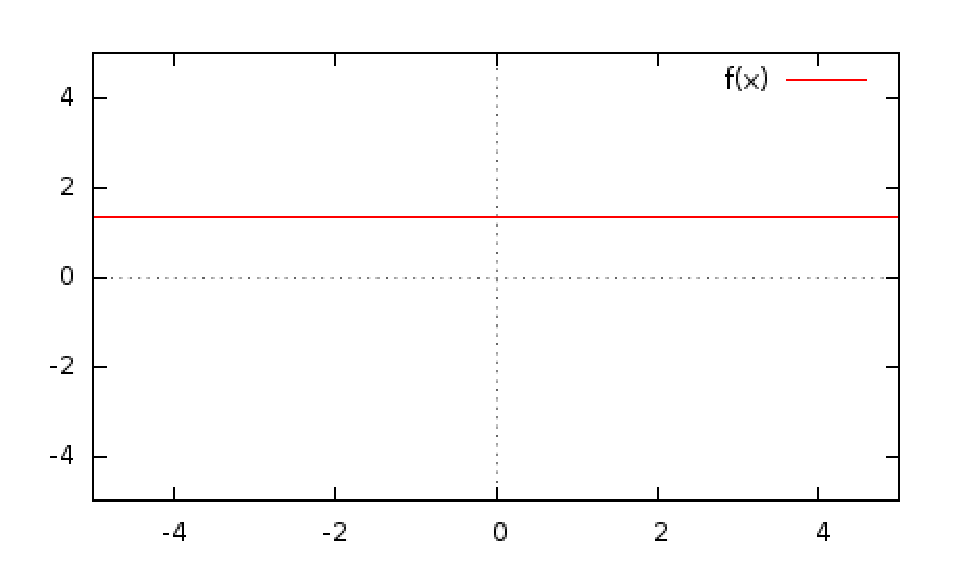
\includegraphics[height=4cm,width=6cm]{fconst.eps} 
\end{center}
\end{minipage}
\hfill



\end{document}
